\chapter{Обзор существующих решений рассматриваемой задачи или её модификаций}
\label{cha:ch_2}

В этой части работы будут кратко описаны методы, применяющиеся при детектировании скоплений на 
микроволновых и рентгеновских данных, а также выбранная нейросетевая архитектура для сегментации 
данных.\\



\section{U-net: нейросетевая архитектура для сегментации данных}
U-net \cite{Unet} является стандартной архитектурой для сегментации данных. Она идеально подходит 
для проверки идеи использования методов глубокого обучения для сегментации скоплений.
Её симметричная структура позволяет абстрагировать данные изображения, подаваемого на 
вход, в то время как skip-connection слои помогают увеличивать точность сегментации.

\begin{figure}[h]
    \center{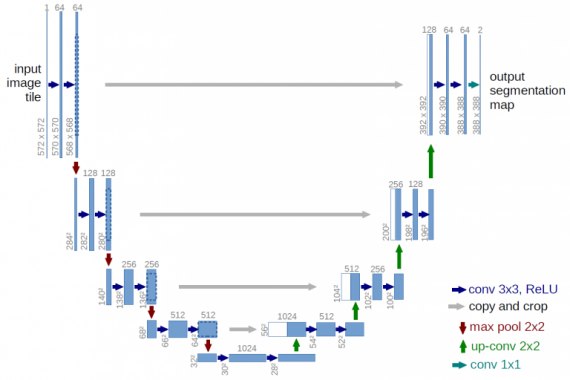
\includegraphics[width=0.7\linewidth]{unet0}}
    \caption{Структура модели U-net \cite{Unet}}
\end{figure}

\section{Сегментация и детекция данных микроволнового диапазона}

В первую очередь рассмотрим работу о детекции эффекта Сюняева-Зельдовича \cite{Bonjean} в 
микроволновых данных. Её автор тоже использует для сегментации данных архитектуру U-net. \\

Основной целью описываемой работы являлось создание алгоритма для детекции источников через эффект 
Сюняева-Зельдовича по данным телескопа <<Планк>>. Соответственно, кроме самих обзоров неба, полученных 
<<Планком>>, использовались еще три ранее упомянутых каталога скоплений для создания целевых данных:

\begin{itemize}
	\item PSZ2 
	\item MCXC 
	\item RedMaPPer 
\end{itemize}

Несмотря на то, что в этих каталогах содержатся данные об объектах, детектированных в разных 
диапазонах, они содержат довольно большое количество общих объектов (поэтому при создании 
тренировочных выборок нужно удалять из каталогов повторы). \\

В описываемой работе для создания тренировочных выборок использовалось разбиение неба проекцией 
HEALPix (Hierarchical Equal Area isoLatitude Pixelisation). \\
\begin{figure}[h]
	\center{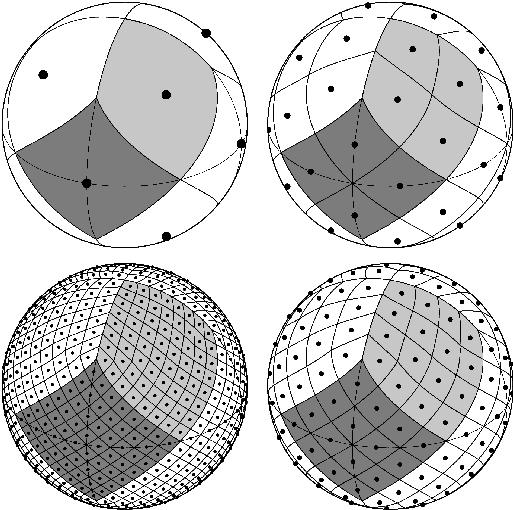
\includegraphics[width=5cm]{healpix0}}
	\caption{Примеры разбиения сферы HEALPix \cite{Healpix}}
\end{figure}

Разбиение с параметром $n_{side}=2$ позволяет получить 48 больших областей неба. Некоторые из них 
были использованы для тестирования полученной модели и для валидации, все остальные были 
использованы для обучения модели.\\ 

Случайным образом в соответствуюхих областях разбиения HEALPix выбирались центры патчей и их 
ориентации для создания тренировочных, валидационных и тестовых выборок. Каждый патч представлял 
из себя изображение размера 64 x 64 с шестью каналами различных данных. Размер каждого пикселя 
на таких патчах составлял 1.7 arcmin. \\

После этого 100000 патчей были использованы для обучения нейросети. Обучение длилось более 30 эпох. \\ 
\begin{figure}[h!]
	\center{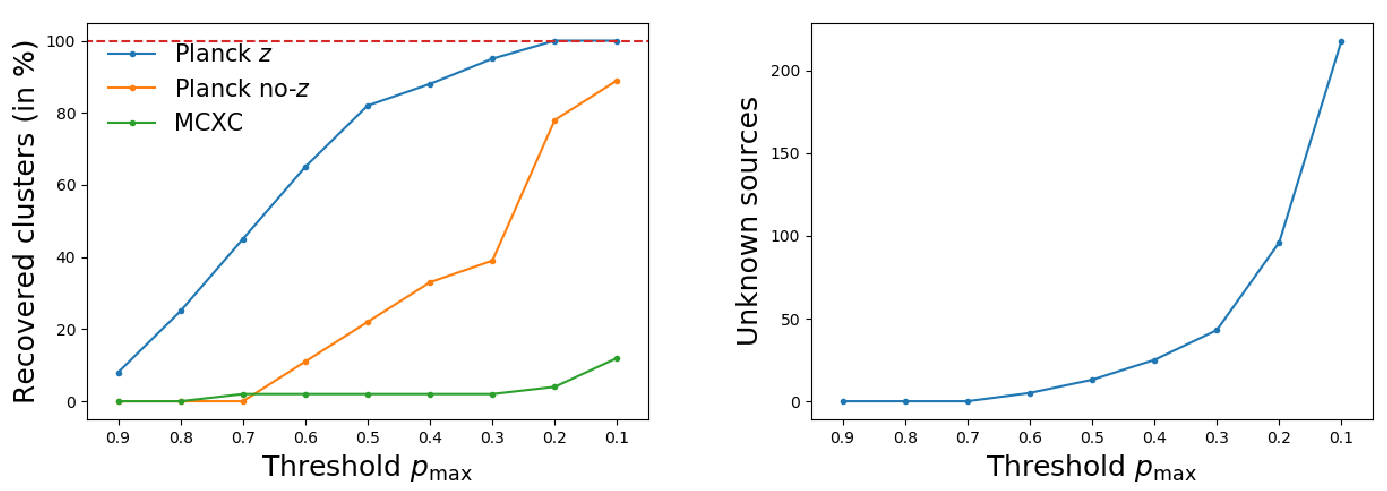
\includegraphics[width=15cm]{sz0}}
	\caption{Результаты исследования работы \cite{Bonjean}}
\end{figure}

Как можно увидеть из результатов, лучше всего нейросеть сегментирует в данных телескопа <<Планк>> 
скопления из каталога того же самого <<Планка>>.\\

В описываемой статье использовалась классическая версия архитектуры U-net: каждый из блоков 
кодировщика состоит из двух свёрток с ядром 3 x 3 с последующими активациями ReLU после каждой 
свёртки за ними следует слой MaxPooling для уменьшения размерности входных данных. Всего в 
кодировщике пять таких блоков. Блоки декодировщика состоят из слоя Upsampling, повышающего 
размерность предыдущего слоя, конкатенации выхода из кодировщика с соответсвующими размерами и 
так же двух сверток с ReLU. Кроме того, после каждого слоя свёртки добавлен слой Dropout с 
параметром 0.2 для предотвращения переобучения. После всех блоков декодировщика добавляется слой 
активации сигмоиды для последующего использования кросс-энтропии как loss-функции. Количество 
фильтров для первого блока варьировалось от 8 до 128.\\

Для детекции скоплений на полученных из нейросети данныx, зонами скоплений обозначались зоны, 
занимающие пиксели со значением больше $p_{max}$, а затем на них находились барицентры, которые 
впоследствии считались предсказанными центрами скоплений. Таким образом большая часть скоплений из 
каталога PSZ2 была успешно распознана нейросетью. \\

\section{Сегментация и детекция данных рентгеновского диапазона}

На данный момент существует несколько пакетов программ, с помощью которых осуществляется 
сегментация данных, полученных с помощью рентгеновских телескопов. Одним из них является CIAO 
(CHANDRA INTERACTIVE ANALYSIS OF OBSERVATIONS), разработанный специально для Космической 
рентгеновской обсерватории «Чандра». \\

\begin{figure}[h]
    \center{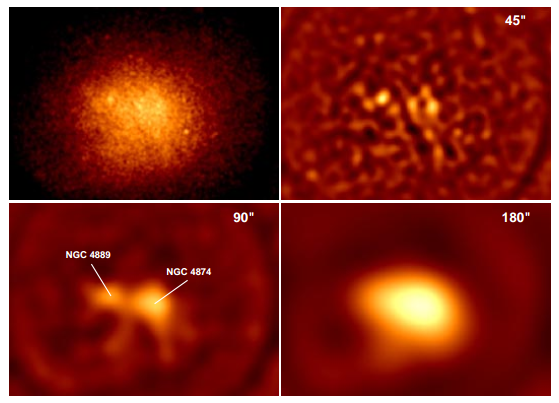
\includegraphics[width=10cm]{wav0}}
    \caption{Вэйвлет-анализ скопления Кома. Сырое изображение и изображение с применёнными 
        к нему вэйвлет-преобразованиями с разным масштабом \cite{Vikhlinin}}
\end{figure}

\begin{itemize}
    \item $celldetect$ использует свёртку с изменяющимся размером ядра для сегментации. Для каждого
        положения клетки вычисляется отношение сигнал/шум, сравнивается со средним значением для 
        фона, и если оно больше, то регистрируется источник, в котором может находится объект.
    \item $vtpdetect$ использует обнаружение источников с помощью тесселяции и перколяции Вороного 
        (VTP) для определения индивидуальных плотностей или потоков для каждого данного пикселя. 
        Затем инструмент анализирует распределение плотностей для обнаружения объектов.
    \item $wavdetect$ использует свёртку вэйвлет функции с астрономических изображением. Такое 
		преобразование позволяет удалить с изображения фон и локализовать структуры, размеры 
		которых близки к масштабу вейвлет-преобразования.
\end{itemize}

Каждый из упомянутых методов является ситуативным и может проявлять себя по-разному для разных 
данных. Все эти методы используют усреднённые рентгеновские данные и не учитывают характеристики 
отдельных телескопов.\\

